% Encoding: UTF-8
% chktex-file 36 % disable -, --, --- check
% chktex-file 18
% chktex-file 16

% Use this if you generate the presentation itself.
\documentclass[final, english, xcolor=pdftex, dvipsnames, handout, table, aspectratio=169, 14pt]{beamer}

% Use this documentclass line for generating the handout
% \documentclass[final, english, xcolor=pdftex, dvipsnames, table, handout, aspectratio=169]{beamer}

\usepackage[utf8]{inputenc}
\usepackage[english]{babel}
\usepackage[T1]{fontenc}
\usepackage{droid}
\pdfmapfile{+droid.map}
\usepackage{fontawesome}
\pdfmapfile{+fontawesome.map}

\usepackage{pgfpages}

% Set the right notes display after your preference
\setbeameroption{hide notes}
%\setbeameroption{show notes}
%\setbeameroption{show notes on second screen=right}
% \setbeameroption{show only notes}

\setbeamerfont{note date}{size=\scriptsize}
\setbeamerfont{note title}{size=\footnotesize}
\setbeamerfont{note page}{size=\footnotesize}

\usepackage{graphicx}

\usepackage[outputdir=build, cachedir=build]{minted}
\usemintedstyle{borland}

\usetheme{DarkConsole}

\graphicspath{./pictures/}

\begin{document}

% The metadata of the presentation
\title[Phonograph]{Phonograph - Chromecast support}
% \subtitle[]{}
\author[]{Markus Pöschl\footnote{\faGithub \ Poeschl \, \faTwitter \ Mr\_Poeschl}}
\date{2018-10-09} % Replace with date of the presentation


\begin{frame}
\maketitle
\end{frame}

\section*{Overview}
\begin{frame}{Overview} % This is the list of content with all the sections of the presentation
\tableofcontents
\end{frame}

\section{What is Phonograph?}

\begin{frame}{What is Phonograph?}

\begin{block}{}
\begin{columns}[onlytextwidth,T]
\column{\dimexpr\linewidth/2}

\textit{Phonograph is a}
\begin{itemize}
  \item Minimalistic
  \item Materialdesigned
  \item Simple
  \item (Folder based)
  \item Open source
\end{itemize}
\textit{music player}

\column{\dimexpr\linewidth/2}
\centering
\includegraphics[width=100px]{pictures/icon_web.png}
\end{columns}
\end{block}
\vspace{20px}

\centering\faGithub \, \normalsize https://github.com/kabouzeid/Phonograph

\note{
\begin{itemize}
  \item Minimalistic
  \item Materialdesigned
  \item Simple
  \item (Folder based)
  \item Open source
\end{itemize}
developed from kabouzeid
}
\end{frame}

\begin{frame}{Screenshots}

\centering
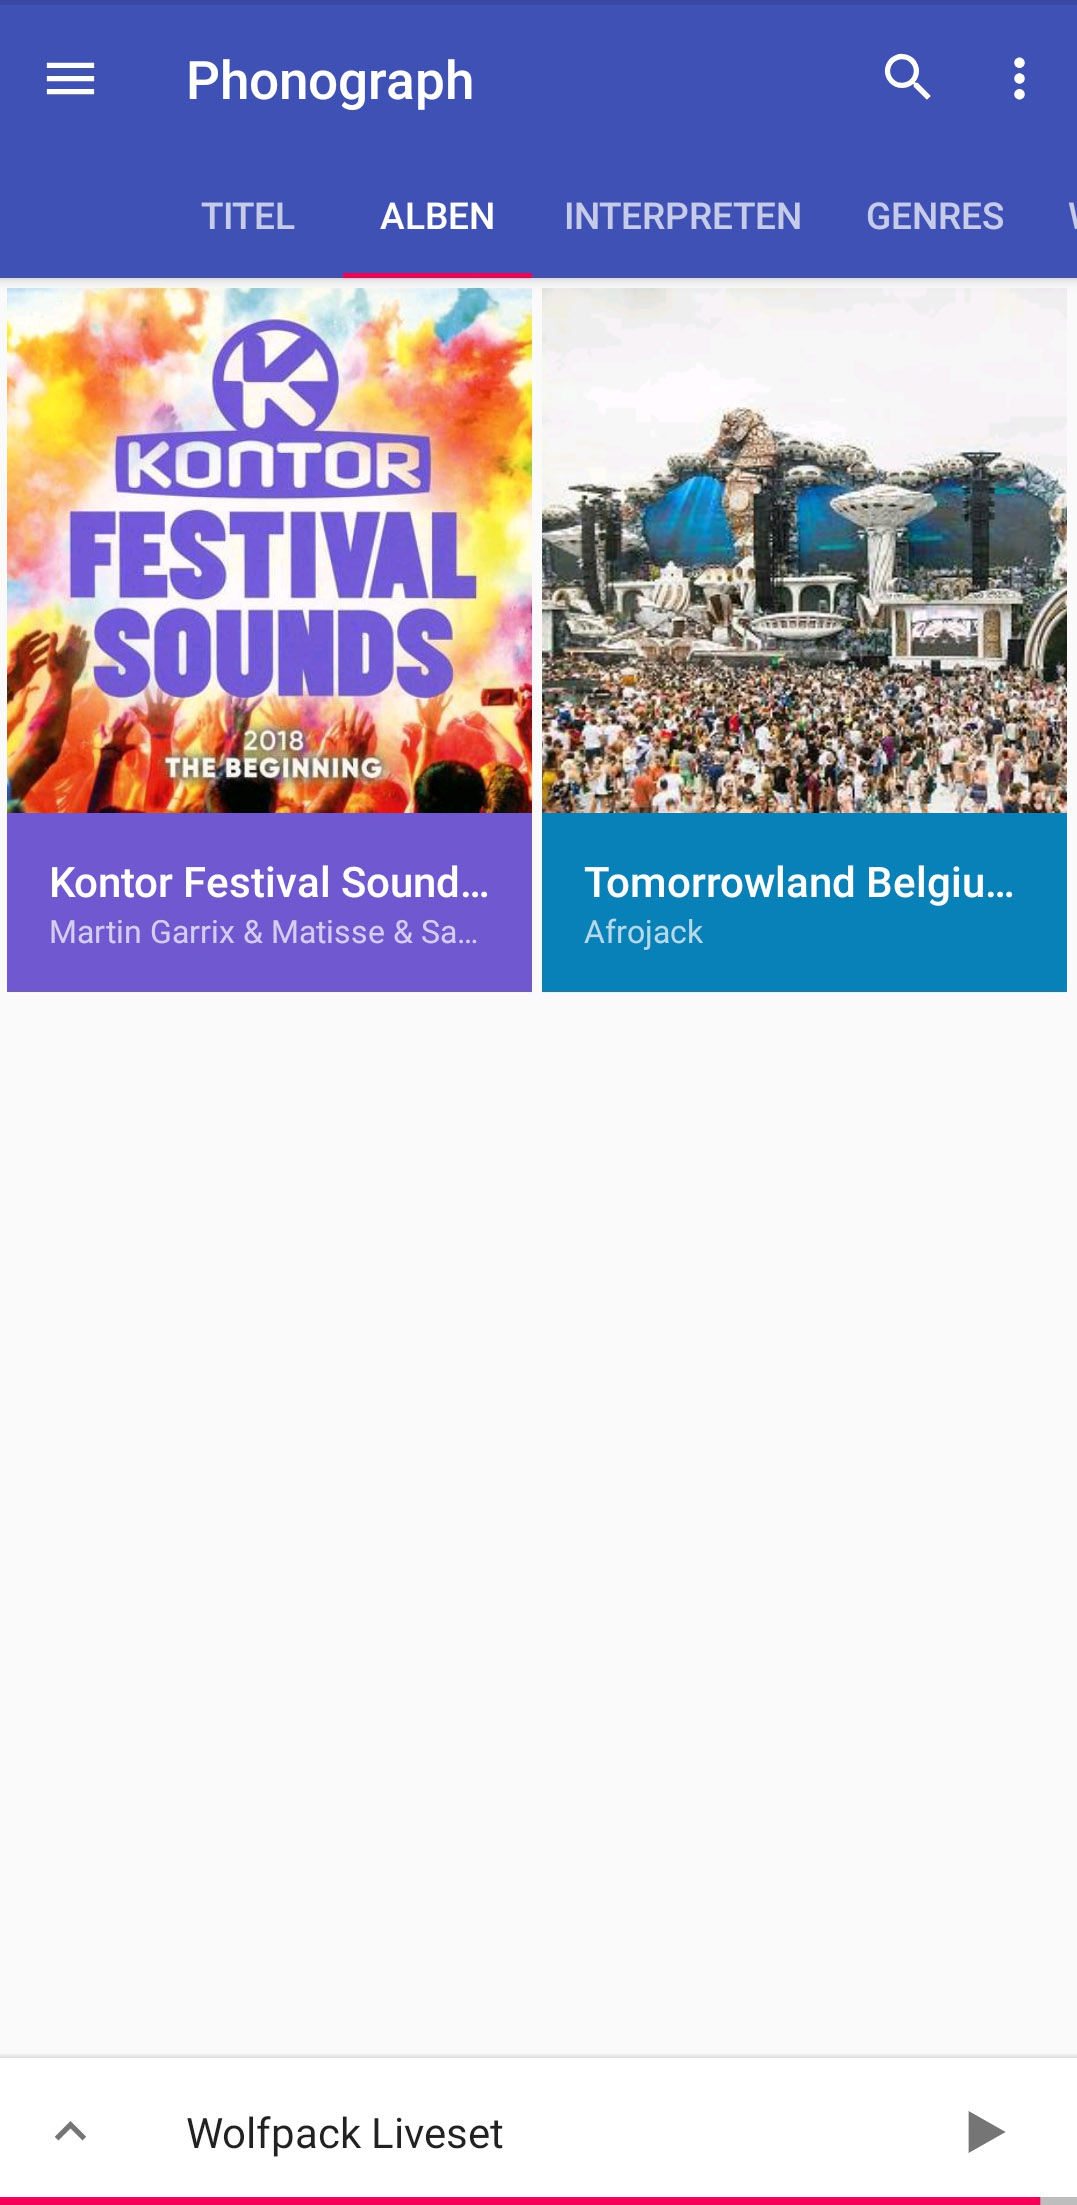
\includegraphics[height=200px]{pictures/Library.jpg} 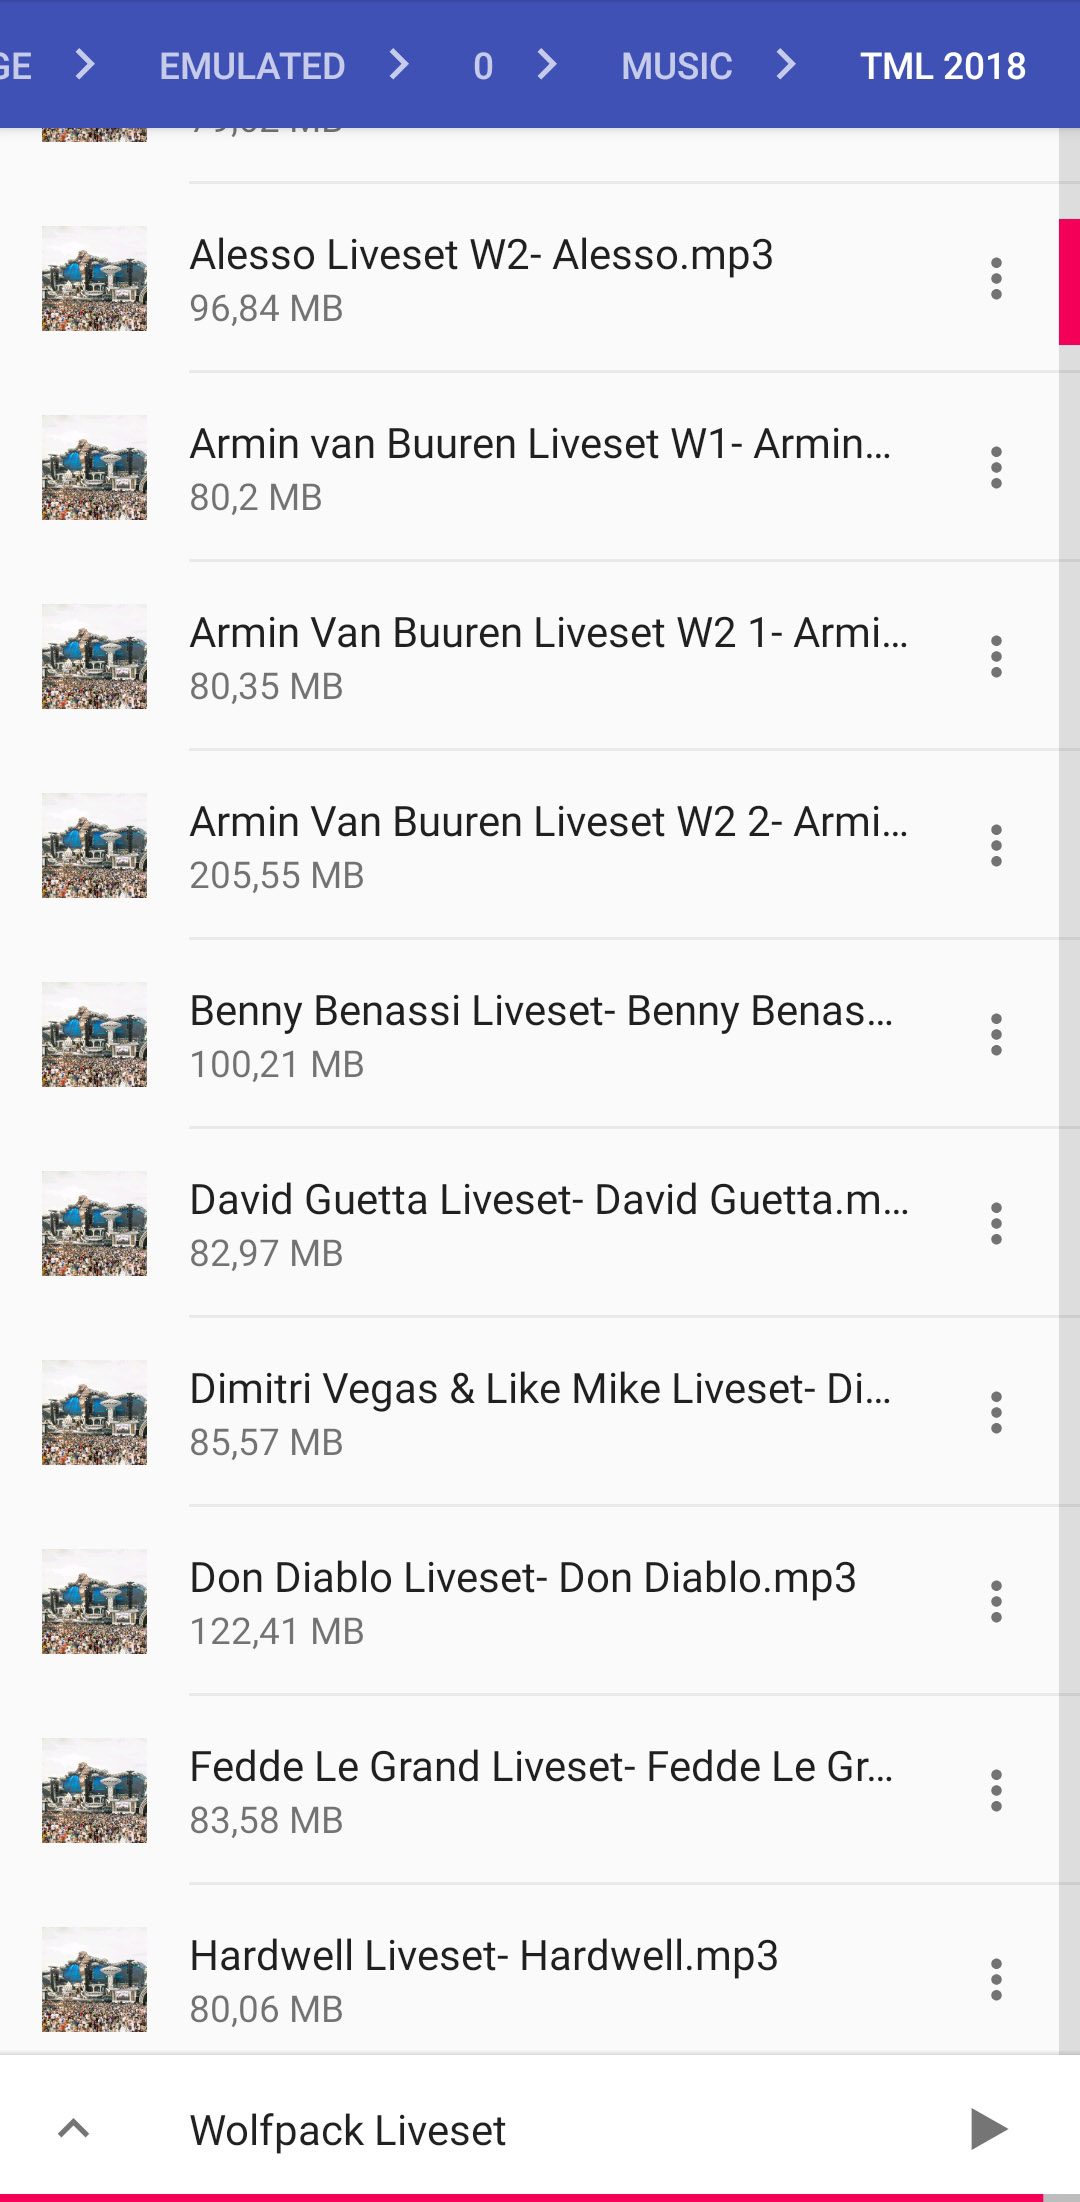
\includegraphics[height=200px]{pictures/Folders.jpg} 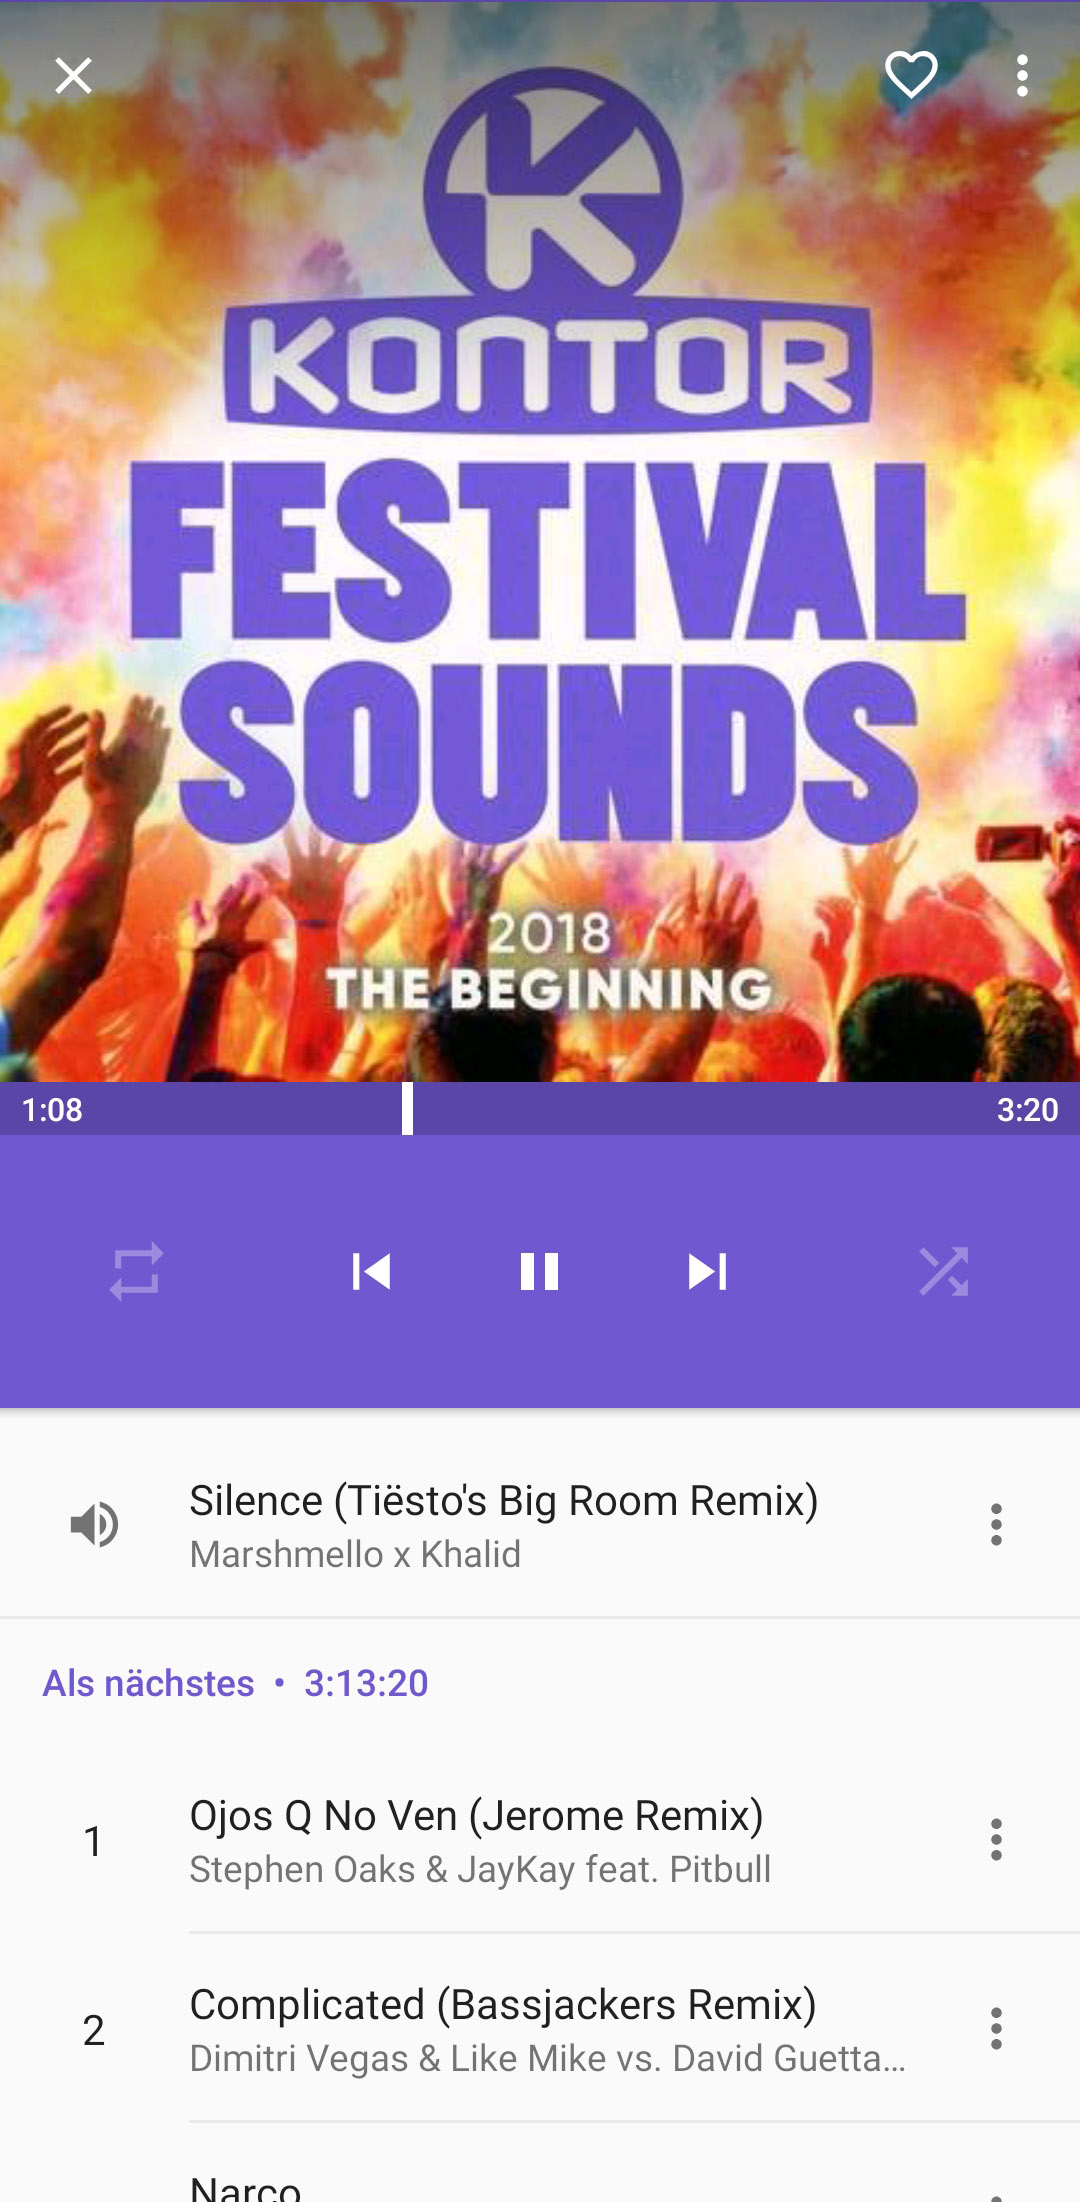
\includegraphics[height=200px]{pictures/Player.jpg}

\note{
\begin{itemize}
  \item Simple Library
  \item Folder based music selection
  \item player interface
\end{itemize}
}
\end{frame}

\section{The Idea for Contribution}

\begin{frame}[c]{Chromecast}

\centering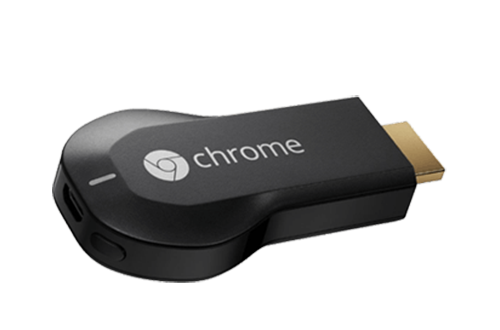
\includegraphics[height=80px]{pictures/chrome-cast-old-image.png}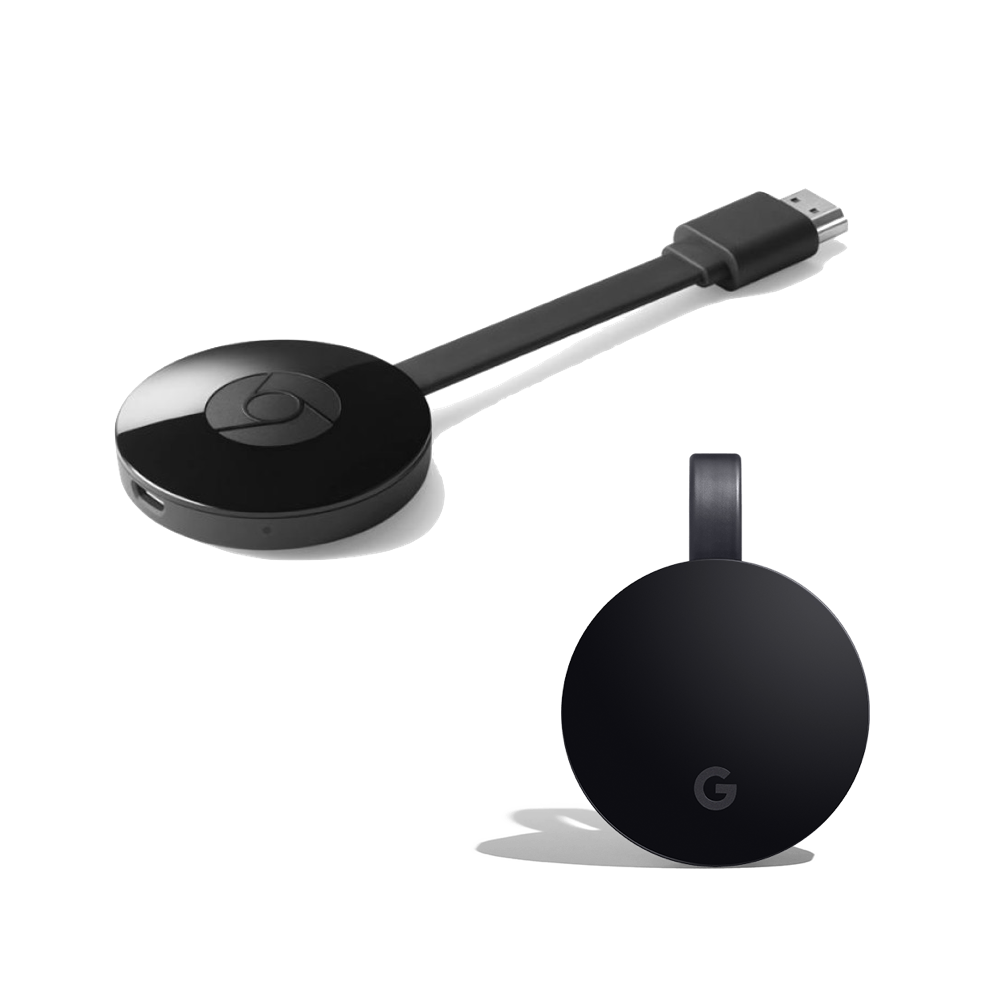
\includegraphics[height=200px]{pictures/chrome-cast-image.png}

\note{
\begin{itemize}
  \item Chromecast is a reciever for media
  \item Fully controlled by a other device
  \item Connected by HDMI and USB
  \item *Show chromecast
\end{itemize}
}
\end{frame}

\begin{frame}{Chromecast Support}
\begin{block}{}
\begin{columns}[onlytextwidth,c]
\column{\dimexpr\linewidth/3}
\centering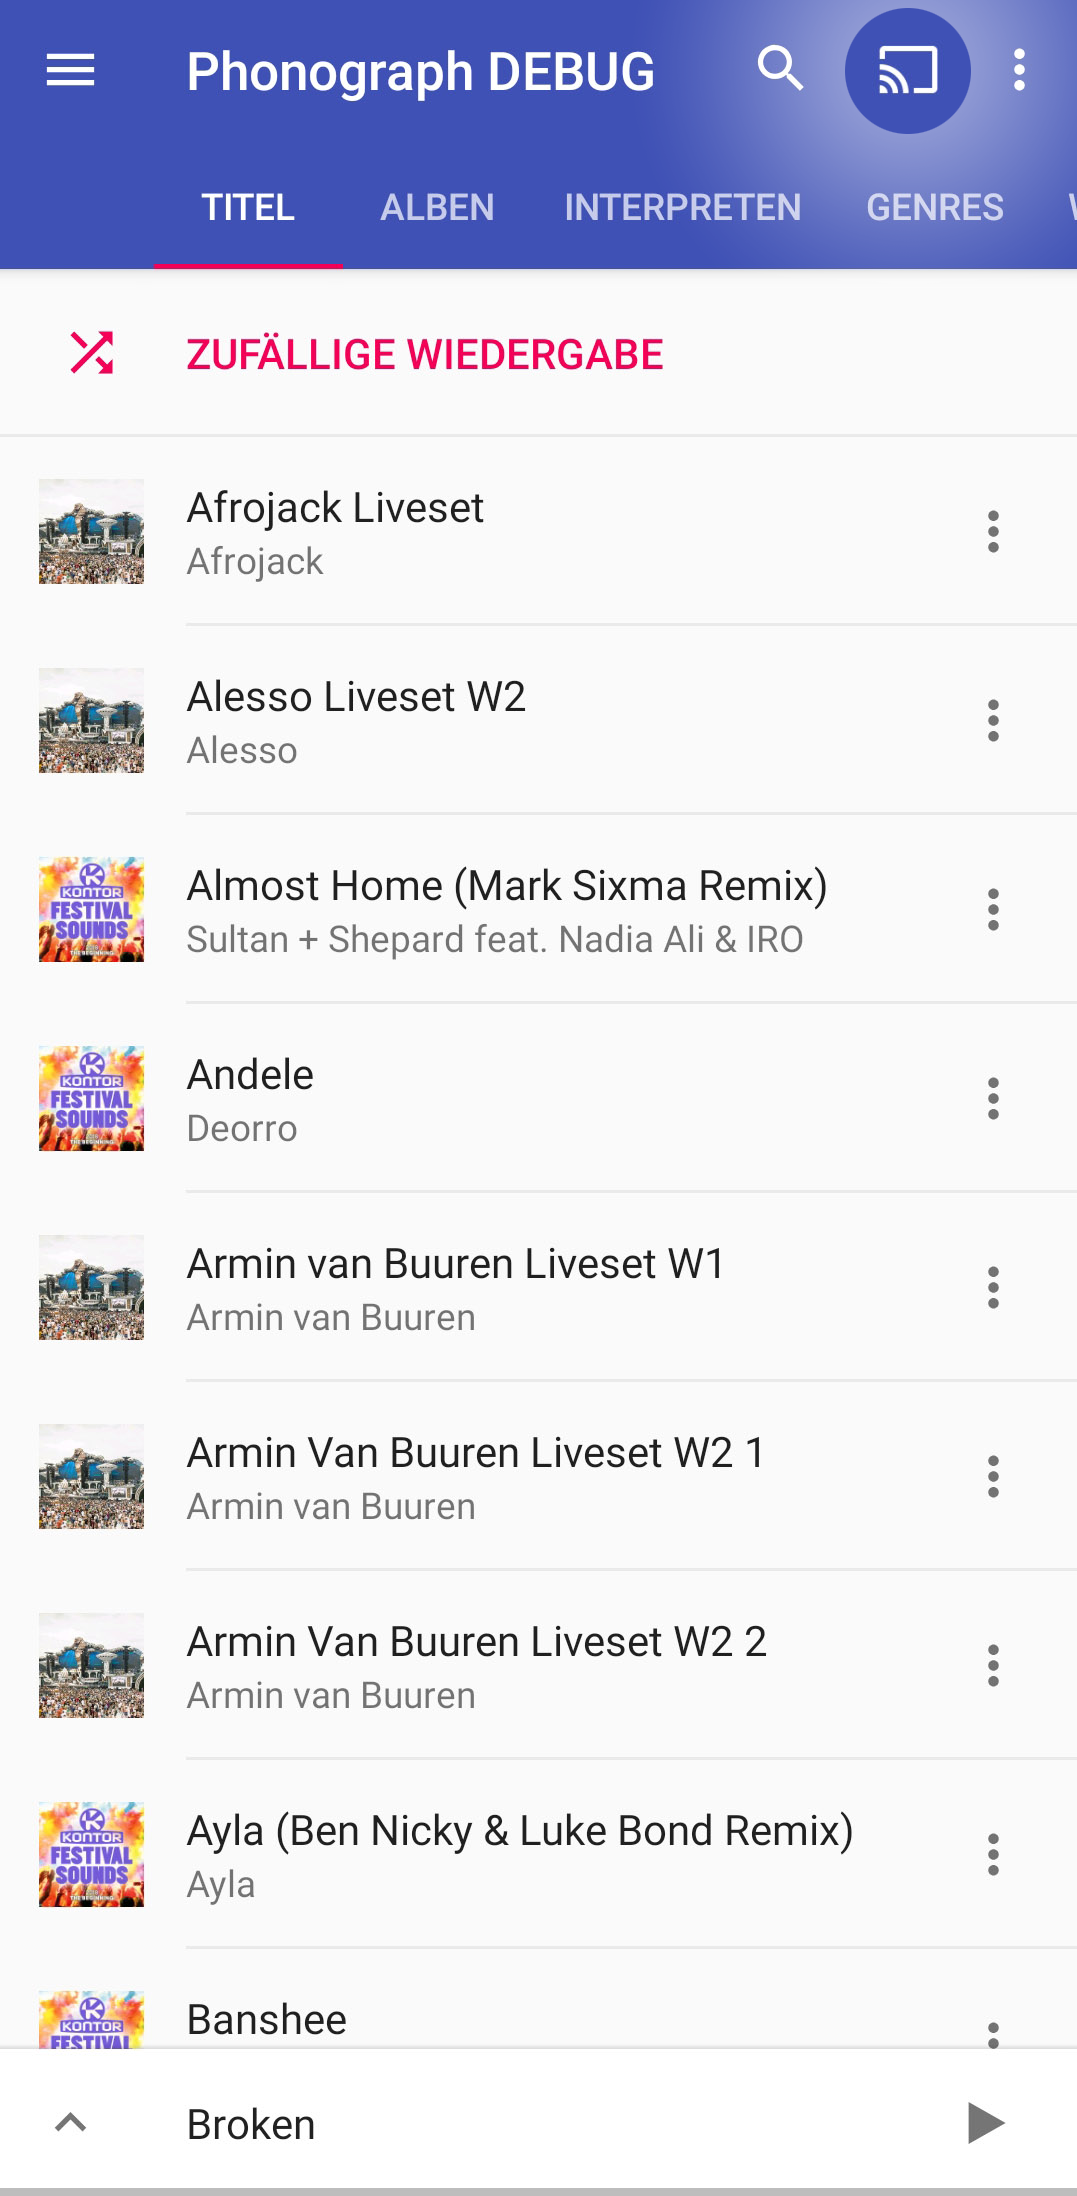
\includegraphics[height=180px]{pictures/Cast-Icon.png}
\column{\dimexpr\linewidth/3}
\centering\huge\faArrowRight
\column{\dimexpr\linewidth/3}
\centering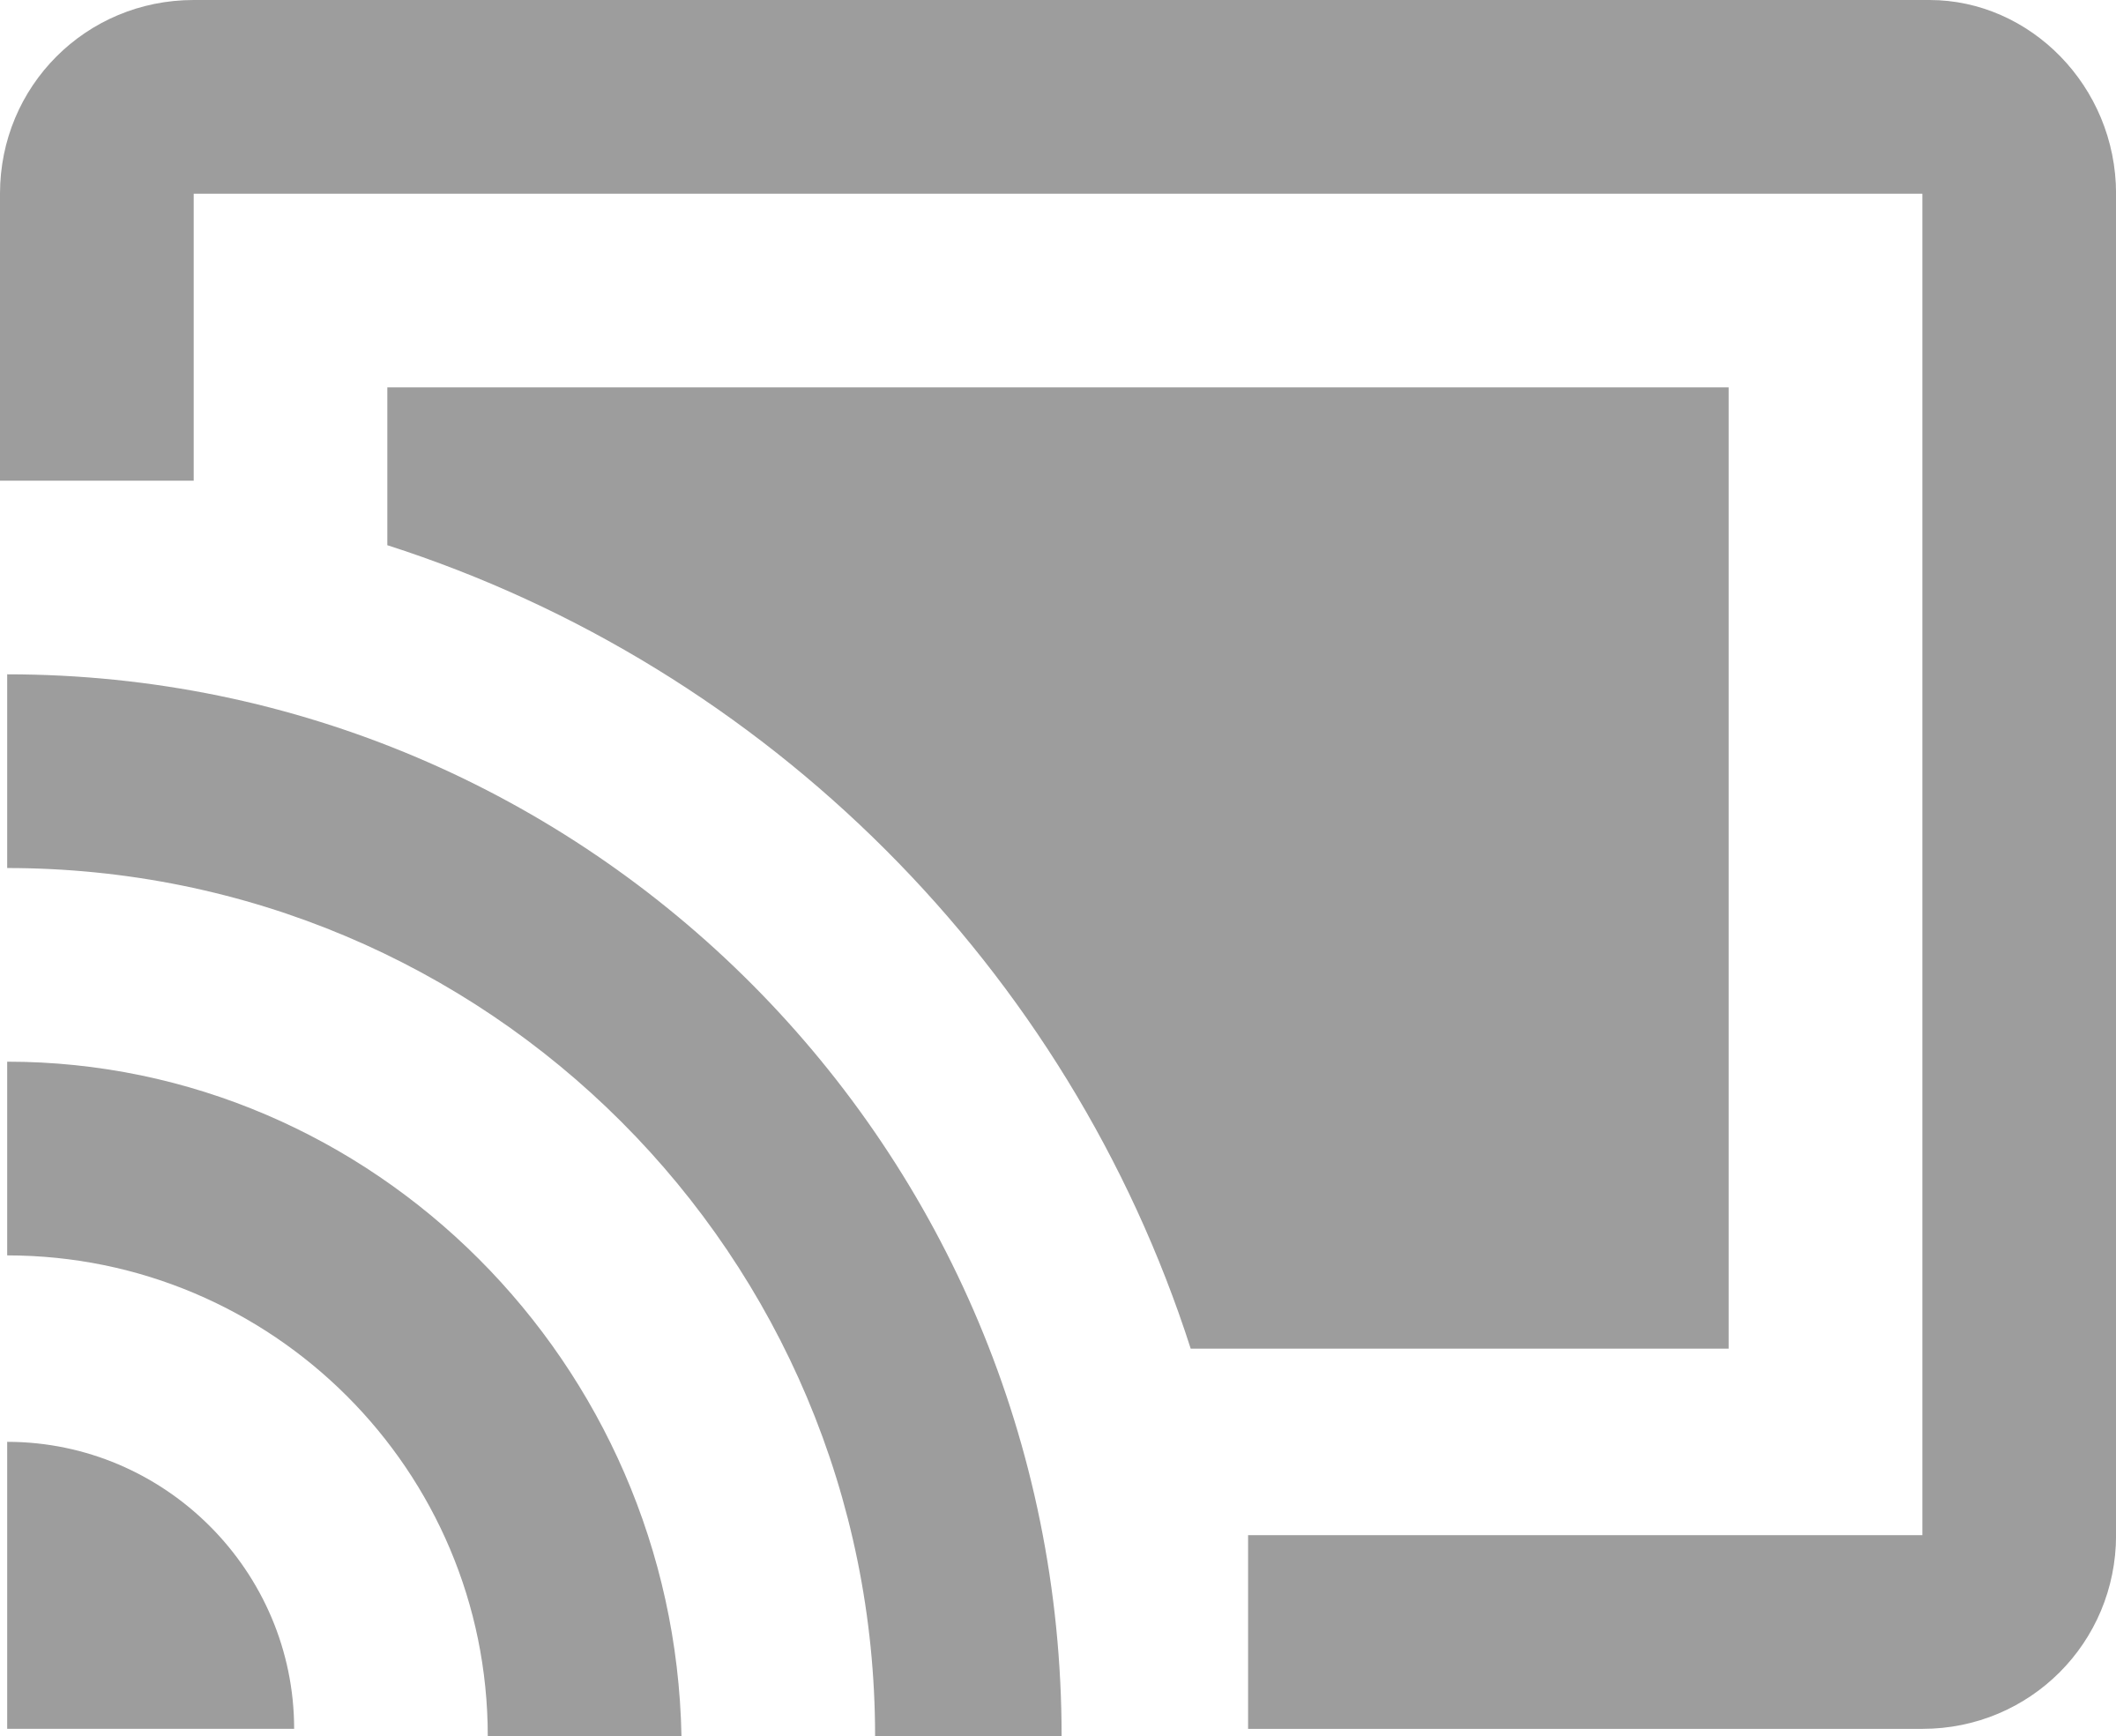
\includegraphics[height=40px]{pictures/chrome-cast.png}
\end{columns}
\end{block} 

\note{
\begin{itemize}
  \item Listening to music
  \item Coming home
  \item Just continue on a chromecast device
\end{itemize}
}
\end{frame}

\begin{frame}{Current Status}

\faCheck \, What is done / started?
\begin{itemize}
  \item Connect with Chromecast (Done)
  \item Play online music on Chromecast (Prototype)
  \item Open local http server to serve music
\end{itemize}\

\faHourglassHalf \, What is on the list?
\begin{itemize}
  \item Serve music files / track images
  \item Integrate the "Cast way" into phonograph\\(this might be a big one)
\end{itemize}

\note{
\begin{itemize}
  \item Connect with Chromecast - Done
  \item Play online music - minimal Prototype
  \item Local http server - doing
  \item todo - serve images
  \item todo - integrate into full (messy) app 
\end{itemize}
}
\end{frame}

\begin{frame}{Source Code}

\centering
\huge\faGithub\\\normalsize https://github.com/Poeschl/Phonograph\

\huge\faCodeFork\\\normalsize chromecast

\note{
Sourcecode at https://github.com/Poeschl/Phonograph/tree/chromecast
}
\end{frame}

\section*{System.exit()}

\begin{frame}{System.exit()}
Thank you for your time.

\vspace{\baselineskip}Questions?

\only<2> {
\vspace{1.5\baselineskip}
\textcolor{gray}{\$ shutdown -h now}
}
\end{frame}

\end{document}
